\documentclass[12pt]{article}\usepackage[]{graphicx}\usepackage[]{color}
%% maxwidth is the original width if it is less than linewidth
%% otherwise use linewidth (to make sure the graphics do not exceed the margin)
\makeatletter
\def\maxwidth{ %
  \ifdim\Gin@nat@width>\linewidth
    \linewidth
  \else
    \Gin@nat@width
  \fi
}
\makeatother

\definecolor{fgcolor}{rgb}{0.345, 0.345, 0.345}
\newcommand{\hlnum}[1]{\textcolor[rgb]{0.686,0.059,0.569}{#1}}%
\newcommand{\hlstr}[1]{\textcolor[rgb]{0.192,0.494,0.8}{#1}}%
\newcommand{\hlcom}[1]{\textcolor[rgb]{0.678,0.584,0.686}{\textit{#1}}}%
\newcommand{\hlopt}[1]{\textcolor[rgb]{0,0,0}{#1}}%
\newcommand{\hlstd}[1]{\textcolor[rgb]{0.345,0.345,0.345}{#1}}%
\newcommand{\hlkwa}[1]{\textcolor[rgb]{0.161,0.373,0.58}{\textbf{#1}}}%
\newcommand{\hlkwb}[1]{\textcolor[rgb]{0.69,0.353,0.396}{#1}}%
\newcommand{\hlkwc}[1]{\textcolor[rgb]{0.333,0.667,0.333}{#1}}%
\newcommand{\hlkwd}[1]{\textcolor[rgb]{0.737,0.353,0.396}{\textbf{#1}}}%

\usepackage{framed}
\makeatletter
\newenvironment{kframe}{%
 \def\at@end@of@kframe{}%
 \ifinner\ifhmode%
  \def\at@end@of@kframe{\end{minipage}}%
  \begin{minipage}{\columnwidth}%
 \fi\fi%
 \def\FrameCommand##1{\hskip\@totalleftmargin \hskip-\fboxsep
 \colorbox{shadecolor}{##1}\hskip-\fboxsep
     % There is no \\@totalrightmargin, so:
     \hskip-\linewidth \hskip-\@totalleftmargin \hskip\columnwidth}%
 \MakeFramed {\advance\hsize-\width
   \@totalleftmargin\z@ \linewidth\hsize
   \@setminipage}}%
 {\par\unskip\endMakeFramed%
 \at@end@of@kframe}
\makeatother

\definecolor{shadecolor}{rgb}{.97, .97, .97}
\definecolor{messagecolor}{rgb}{0, 0, 0}
\definecolor{warningcolor}{rgb}{1, 0, 1}
\definecolor{errorcolor}{rgb}{1, 0, 0}
\newenvironment{knitrout}{}{} % an empty environment to be redefined in TeX

\usepackage{alltt}

\usepackage{amssymb,amsmath}
\usepackage{enumerate}
\usepackage{float}
\usepackage{verbatim}
\usepackage{setspace}
\usepackage{graphicx, multicol}

%% LaTeX margin settings:
  \setlength{\textwidth}{7.0in}
\setlength{\textheight}{9in}
\setlength{\oddsidemargin}{-.5in}
\setlength{\evensidemargin}{0in}
\setlength{\topmargin}{-1.5cm}

%% tell knitr to use smaller font for code chunks
\def\fs{\footnotesize}
\def\R{{\sf R}}
\newcommand{\bfbeta}{\mbox{\boldmath $\beta$}}
\newcommand{\bfD}{\mbox{\boldmath $D$}}
\newcommand{\bfL}{\mbox{\boldmath $L$}}
\newcommand{\bfR}{\mbox{\boldmath $R$}}
\newcommand{\bfmu}{\mbox{\boldmath $\mu$}}
\newcommand{\bfv}{\mbox{\boldmath $V$}}
\newcommand{\bfX}{\mbox{\boldmath $X$}}
\newcommand{\bfy}{\mbox{\boldmath $y$}}
\newcommand{\bfb}{\mbox{\boldmath $b$}}
\IfFileExists{upquote.sty}{\usepackage{upquote}}{}
\begin{document}


  
  
\begin{center}
\large{Bayes: Homework $9$} \\
Leslie Gains-Germain
\end{center}

\begin{doublespacing}

\begin{enumerate}

\item \begin{enumerate}

\item \begin{enumerate}

\item Scenario 1: three chains from $N(0, 1)$ white noise. I actually ran $2000$ iterations in each chain so that I could use Raftery and Lewis's diagnostic in part (e).
\begin{center}
\begin{knitrout}\footnotesize
\definecolor{shadecolor}{rgb}{0.969, 0.969, 0.969}\color{fgcolor}
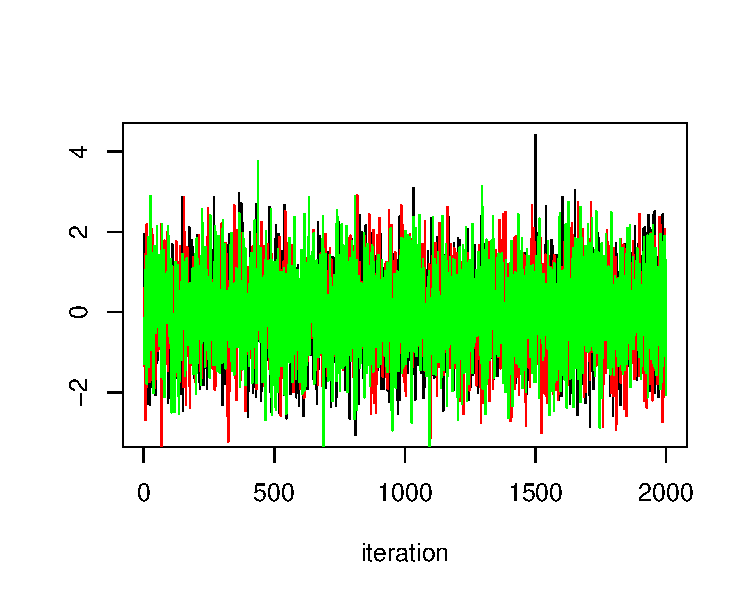
\includegraphics[width=.5\linewidth]{figure/n01} 

\end{knitrout}
\end{center}

\item Scenario 2: one chain from $N(-1, 1)$, one chain from $N(0, 1)$, and one chain from $N(1, 1)$.
\begin{center}
\begin{knitrout}\footnotesize
\definecolor{shadecolor}{rgb}{0.969, 0.969, 0.969}\color{fgcolor}
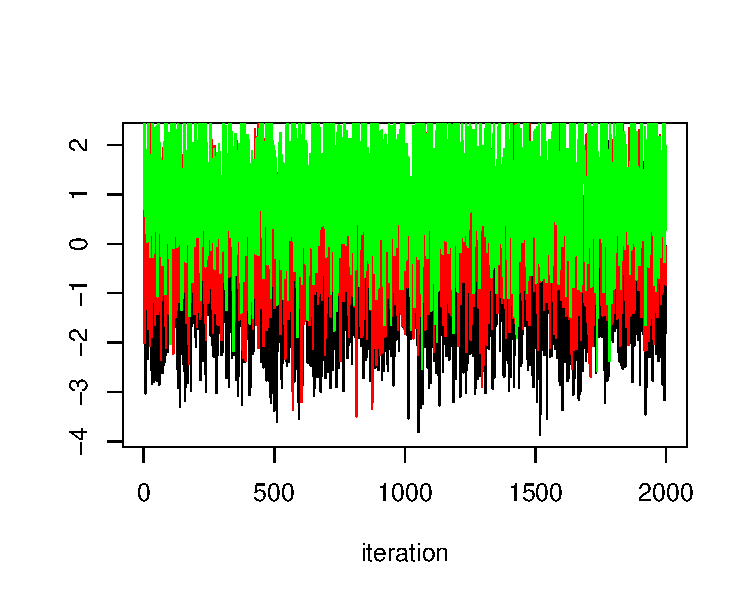
\includegraphics[width=.5\linewidth]{figure/norms} 

\end{knitrout}
\end{center}

\item Scenario 3: three from $MVN(0, \Sigma)$ with common $\sigma^2=1$ and $\rho=0.8$. 
\begin{center}
\begin{knitrout}\footnotesize
\definecolor{shadecolor}{rgb}{0.969, 0.969, 0.969}\color{fgcolor}
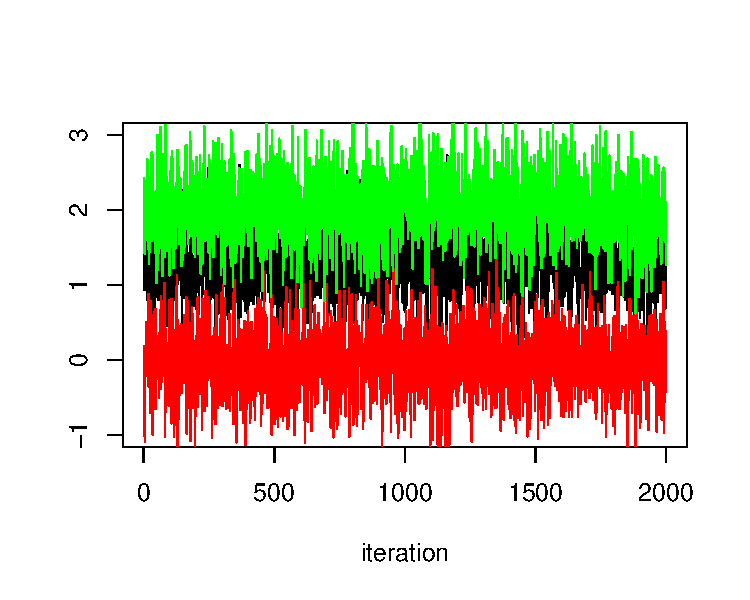
\includegraphics[width=.5\linewidth]{figure/mvnorms} 

\end{knitrout}
\end{center}

\item Scenario 4: three from non-stationary correlated chains using \verb+diffinv(rnorm(999))+.
\begin{center}
\begin{knitrout}\footnotesize
\definecolor{shadecolor}{rgb}{0.969, 0.969, 0.969}\color{fgcolor}
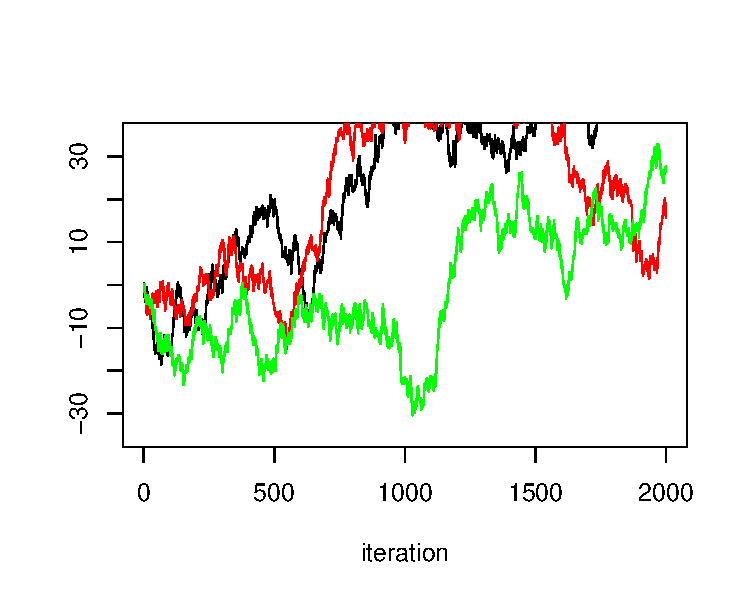
\includegraphics[width=.5\linewidth]{figure/diffinvnorms} 

\end{knitrout}
\end{center}

\item Scenario 5: three from stationary chains with correlation using \\
\verb+filter(rnorm(1000), filter=rep(1, 10), circular=TRUE)+.
\begin{center}
\begin{knitrout}\footnotesize
\definecolor{shadecolor}{rgb}{0.969, 0.969, 0.969}\color{fgcolor}
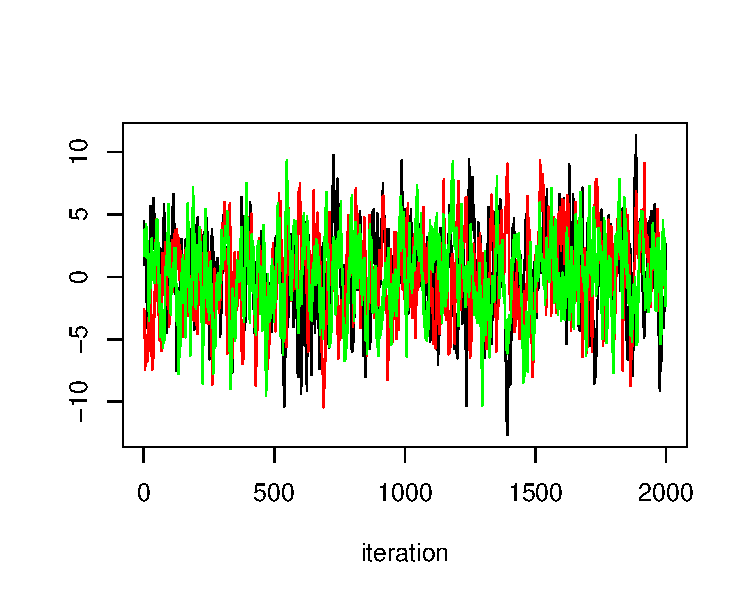
\includegraphics[width=.5\linewidth]{figure/statinvnorms} 

\end{knitrout}
\end{center}

\end{enumerate}

\item The effective sample size is calculated differently in the newest version of the \verb+coda+ package than described in the textbook. In the textbook, the effective sample size is found by dividing the number of iterations (over all chains) by a formula that measures autocorrelation, so that chains with higher autocorrelation have lower effective sample sizes. In the newest version of the \verb+coda+ package, however, the number of iterations is divided by the spectral density. Details are on page $286$ of the BDA3 text and the Effective Sample size section of the convergence diagnostic document. \\

In the coda package, $\hat{R}$ is calculated in the same way as the described in Chapter $11$ in the BDA3 textbook.

\item The below table shows the $\hat{R}$ and effective sample sizes for each scenario.

% latex table generated in R 3.2.1 by xtable 1.7-4 package
% Fri Nov  6 14:51:42 2015
\begin{table}[ht]
\centering
\begin{tabular}{lrr}
  \hline
scenario & neff & rhat \\ 
  \hline
1 & 5674.27 & 1.00 \\ 
  2 & 6291.69 & 1.74 \\ 
  3 & 5526.62 & 3.61 \\ 
  4 & 7.34 & 2.22 \\ 
  5 & 540.03 & 1.00 \\ 
   \hline
\end{tabular}
\end{table}


\item The table below shows the z-statistics for all three chains from Geweke's diagnostic. The last three columns show the results from Raftery and Lewis's diagnostic (burn in and iterations required as well as the dependence factor).

% latex table generated in R 3.2.1 by xtable 1.7-4 package
% Fri Nov  6 14:51:43 2015
\begin{table}[ht]
\centering
\begin{tabular}{lrrrrrr}
  \hline
scenario & zstats1 & zstats2 & zstats3 & burn.in & n.iter & dependence.factor \\ 
  \hline
1 & 0.00 & -1.87 & -0.60 & 2.00 & 3660.00 & 0.98 \\ 
  2 & -0.17 & -1.17 & 0.12 & 3.00 & 4255.00 & 1.14 \\ 
  3 & -2.01 & 0.16 & -0.74 & 3.00 & 4197.00 & 1.12 \\ 
  4 & -11.17 & -3.51 & -2.35 & 198.00 & 215594.00 & 57.60 \\ 
  5 & 0.15 & -2.19 & -0.09 & 20.00 & 21264.00 & 5.68 \\ 
   \hline
\end{tabular}
\end{table}


\item Convergence in Scenario $1$ looks good - there is little autocorrelation within chains, and the between chain variability is low. Scenario $2$ has little autocorrelation within chains, but large between chain variability. Scenario $3$ looks similar to Scenario $2$, but I think something might have gone wrong (see discussion below). Scenario $4$ has both high correlation within chains and large between chain variability. Scenario $5$ has small between chain variability but high correlation within chains. \\

I am confused about Scenario $3$ and worried that I coded the simulations wrong. This scenario is supposed to be three chains with high correlation among the draws within each chain. But, for some reason, the chains get stuck in the part of the parameter space where they start. I would have expected to see a traceplot more similar to Scenario $4$. Below is the code I used for Scenario $3$:
\begin{singlespace}
\begin{knitrout}\footnotesize
\definecolor{shadecolor}{rgb}{0.969, 0.969, 0.969}\color{fgcolor}\begin{kframe}
\begin{alltt}
\hlkwd{set.seed}\hlstd{(}\hlnum{321}\hlstd{)}
\hlstd{nsim} \hlkwb{<-} \hlnum{2000}
\hlstd{Sigma} \hlkwb{<-} \hlkwd{diag}\hlstd{(nsim)}
\hlkwd{require}\hlstd{(gdata)}
\hlkwd{upperTriangle}\hlstd{(Sigma)} \hlkwb{<-} \hlnum{0.8}
\hlkwd{lowerTriangle}\hlstd{(Sigma)} \hlkwb{<-} \hlnum{0.8}

\hlkwd{require}\hlstd{(LearnBayes)}
\hlstd{one3} \hlkwb{<-} \hlkwd{c}\hlstd{(}\hlkwd{rmnorm}\hlstd{(}\hlnum{1}\hlstd{,} \hlkwd{rep}\hlstd{(}\hlnum{0}\hlstd{, nsim), Sigma))}
\hlstd{two3} \hlkwb{<-} \hlkwd{c}\hlstd{(}\hlkwd{rmnorm}\hlstd{(}\hlnum{1}\hlstd{,} \hlkwd{rep}\hlstd{(}\hlnum{0}\hlstd{, nsim), Sigma))}
\hlstd{three3} \hlkwb{<-} \hlkwd{c}\hlstd{(}\hlkwd{rmnorm}\hlstd{(}\hlnum{1}\hlstd{,} \hlkwd{rep}\hlstd{(}\hlnum{0}\hlstd{, nsim), Sigma))}
\end{alltt}
\end{kframe}
\end{knitrout}
\end{singlespace}

Geweke's Diagnostic picks up on a problem with Scenario $4$, with large z-statistics for all three chains. Geweke's diagnostic does not, however, does not pick up on the large between chain variability in Scenario $2$. I definitely would not want to use Geweke's diagnostic blindly without looking at a traceplot. Raftery and Lewis's diagnostic picks up on the high within chain correlation for Scenarios $4$ and $5$, but it also does not pick up on large variability between chains in Scenarios $2$ and $3$. \\

I think a main point of this exercise is to notice that it is not enough to look at one convergence diagnostic only. It's important to look at the traceplots and several convergence diagnostics. A good example of this is Scenario $2$. In this scenario, the effective sample size indicates little autocorrelation within the chains, but the $\hat{R}$ value reveals the large amount of between chain variability. If I had only looked at the effective sample size without looking at the traceplots and $\hat{R}$, I wouldn't have known there was a problem with convergence. Another example of this is Scenario $5$. In Scenario $5$, the $\hat{R}$ value is close to $1$, but the effective sample size is low ($540$ out of $2000$ trials), indicating correlation among the chains. Lesson: Always consider several diagnostics and the traceplots when assessing convergence!

{\bf Question: What is the difference between saying a chain is stationary and saying that convergence has been reached?}

\end{enumerate}

\item \begin{enumerate}

\item $\sigma_{\alpha}^2$ is $Inv-Gamma(0.001, 0.001)$ which is the same as a scaled inverse chi squared distribution with parameters $\nu=0.002$ and $s^2=1$.

\item The plots of all the priors are shown below.

\begin{knitrout}\footnotesize
\definecolor{shadecolor}{rgb}{0.969, 0.969, 0.969}\color{fgcolor}
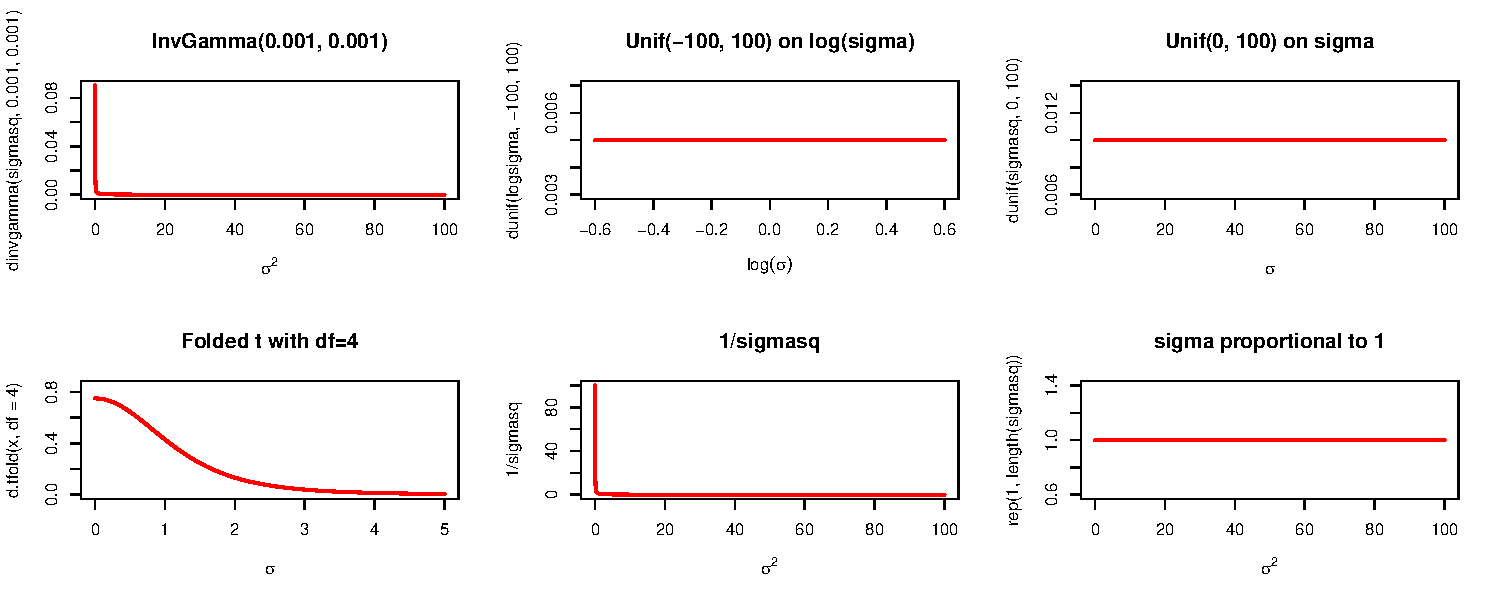
\includegraphics[width=\linewidth]{figure/plotprior1} 

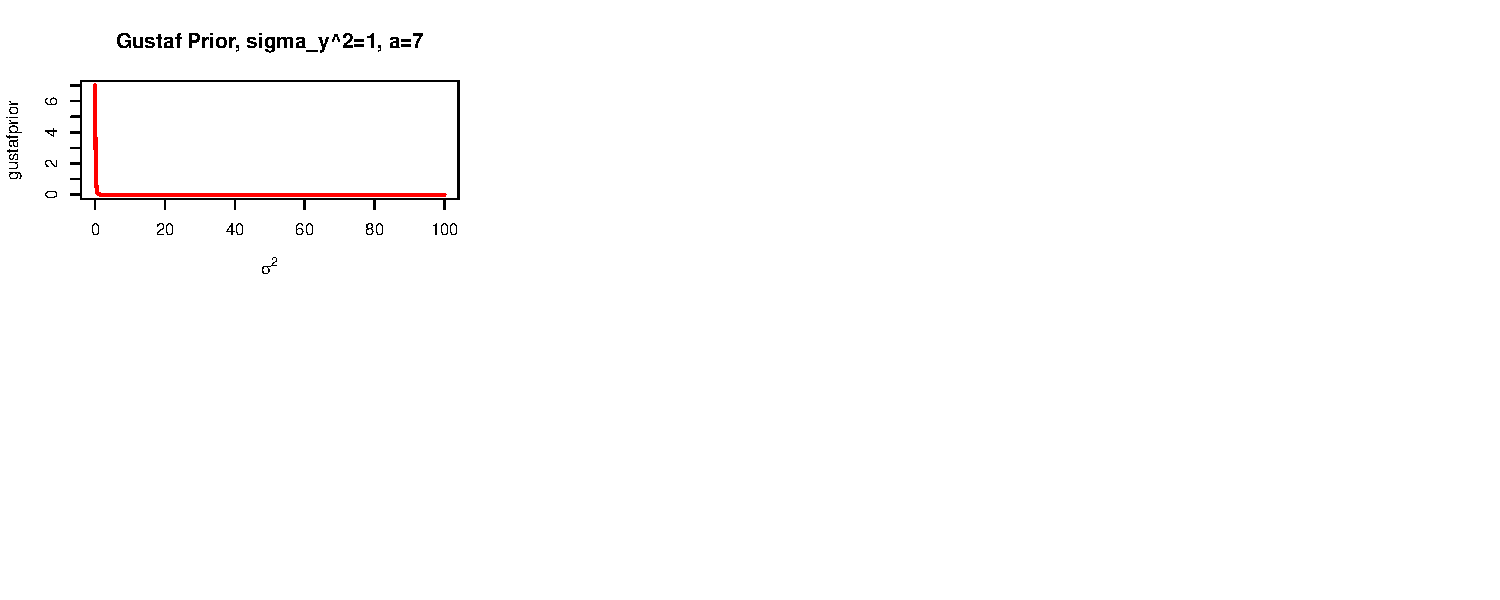
\includegraphics[width=\linewidth]{figure/plotprior2} 

\end{knitrout}

\item I took random draws from prior B and I exponentiated these draws to compare to prior C. Clearly, a prior of $log(\sigma)$ is very different from a uniform prior on $\sigma$. The plot is hard to see, but you can tell that after drawing from a $Unif(-100, 100)$ prior on $log(\sigma)$, you get many very large values for $\sigma$ (not shown), and you get many very very small values for $\sigma$. This is why the $log(\sigma)$ prior blows up at zero. Priors B and C generate very different values for $\sigma$. It makes sense why Gelman recommends a uniform prior on the standard deviation rather than a uniform prior on the log standard deviation.

\begin{center}
\begin{knitrout}\footnotesize
\definecolor{shadecolor}{rgb}{0.969, 0.969, 0.969}\color{fgcolor}
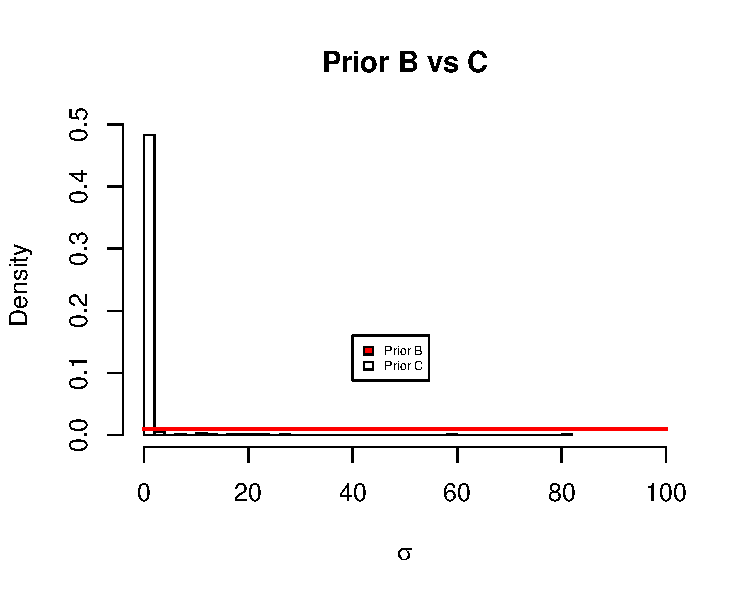
\includegraphics[width=.5\linewidth]{figure/priorsigmatheta} 

\end{knitrout}
\end{center}


\item I took $10000$ random draws from a $Unif(0, 100)$ distribution of $\sigma_{\theta}$, and then I exponentiated these draws to compare to the Inverse Gamma prior on $\sigma_{\theta}^2$. It actually looks like the $Uniform(0, 100)$ prior on $\sigma_{\theta}$ is similar in shape to a $Inv-Gamma(0.001, 0.001)$ prior on $\sigma^2_{\theta}$, but the uniform prior on the standard deviation looks better because although there are many $\sigma^2_{\theta}$ values near $0$, the prior does not blow up at zero like the Inverse Gamma prior does.

\begin{knitrout}\footnotesize
\definecolor{shadecolor}{rgb}{0.969, 0.969, 0.969}\color{fgcolor}
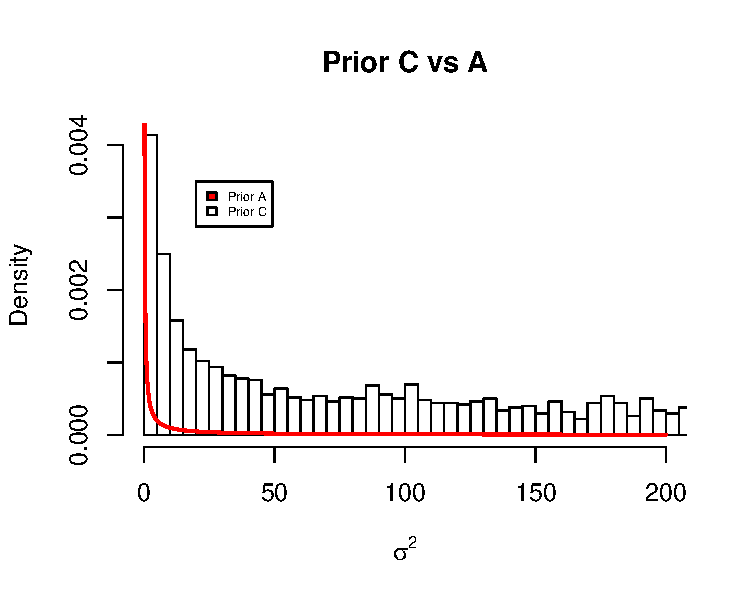
\includegraphics[width=.5\linewidth]{figure/comparecanda} 

\end{knitrout}


\item A half-Cauchy distribution is a half t-distribution with $1$ df. 

\end{enumerate}

\item \begin{enumerate}

\item \begin{enumerate}
\item The \verb+dtfolded+ function below calculates the density of a folded half t distribution with \verb+df+ degrees of freedom and a scale of A.
\begin{center}
\begin{singlespace}
\begin{knitrout}\footnotesize
\definecolor{shadecolor}{rgb}{0.969, 0.969, 0.969}\color{fgcolor}\begin{kframe}
\begin{alltt}
\hlcom{# function to calculate density of a folded non-central t-distribution}
\hlstd{dtfolded} \hlkwb{<-} \hlkwa{function} \hlstd{(}\hlkwc{x}\hlstd{,} \hlkwc{df}\hlstd{=}\hlnum{4}\hlstd{,} \hlkwc{A}\hlstd{=}\hlnum{1}\hlstd{) \{}
  \hlstd{p} \hlkwb{<-} \hlstd{(}\hlnum{1}\hlopt{+}\hlnum{1}\hlopt{/}\hlstd{df}\hlopt{*}\hlstd{(x}\hlopt{/}\hlstd{A)}\hlopt{^}\hlnum{2}\hlstd{)}\hlopt{^}\hlstd{(}\hlopt{-}\hlstd{(df}\hlopt{+}\hlnum{1}\hlstd{)}\hlopt{/}\hlnum{2}\hlstd{)}
  \hlstd{num.int} \hlkwb{<-} \hlkwd{sum}\hlstd{(p}\hlopt{*}\hlstd{(x[}\hlnum{2}\hlstd{]}\hlopt{-}\hlstd{x[}\hlnum{1}\hlstd{]))}
  \hlstd{dt} \hlkwb{<-} \hlstd{p}\hlopt{/}\hlstd{num.int}
  \hlkwd{return}\hlstd{(dt)}
\hlstd{\}}

\hlstd{x} \hlkwb{<-} \hlkwd{seq}\hlstd{(}\hlnum{0}\hlstd{,} \hlnum{20}\hlstd{,} \hlkwc{by}\hlstd{=}\hlnum{0.01}\hlstd{)}

\hlkwd{plot}\hlstd{(x,} \hlkwd{dtfolded}\hlstd{(x),} \hlkwc{type}\hlstd{=}\hlstr{"l"}\hlstd{,} \hlkwc{main}\hlstd{=}\hlstr{"Half-t density"}\hlstd{,} \hlkwc{lwd}\hlstd{=}\hlnum{2}\hlstd{)}
\end{alltt}
\end{kframe}
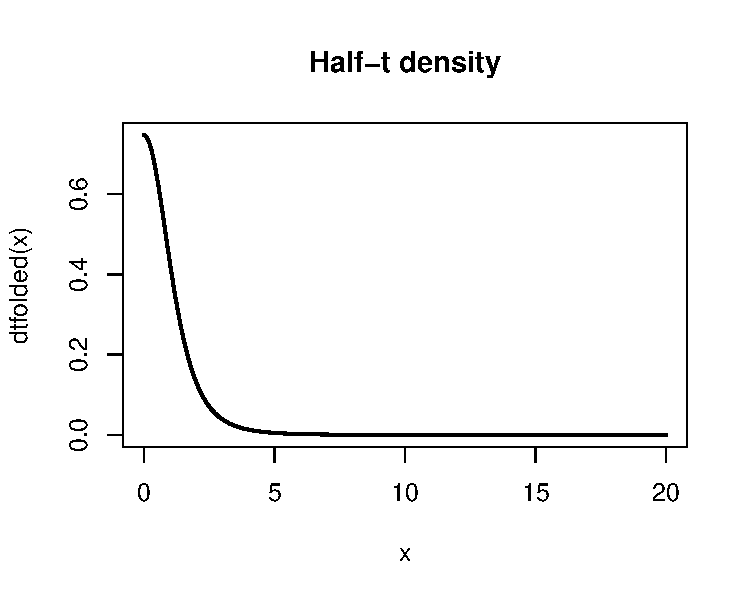
\includegraphics[width=.5\linewidth]{figure/density} 

\end{knitrout}
\end{singlespace}
\end{center}

\item The \verb+rtfolded+ function below generates a random draw from the folded t distribution with \verb+df+ degrees of freedom and scale parameter of A. 
\begin{singlespace}
\begin{center}
\begin{knitrout}\footnotesize
\definecolor{shadecolor}{rgb}{0.969, 0.969, 0.969}\color{fgcolor}\begin{kframe}
\begin{alltt}
\hlstd{rtfolded} \hlkwb{<-} \hlkwa{function}\hlstd{(}\hlkwc{nsim}\hlstd{,} \hlkwc{df}\hlstd{=}\hlnum{4}\hlstd{,} \hlkwc{mu}\hlstd{=}\hlnum{0}\hlstd{,} \hlkwc{sigma}\hlstd{=}\hlnum{1}\hlstd{,} \hlkwc{A}\hlstd{=}\hlnum{3}\hlstd{)\{}
  \hlstd{z} \hlkwb{<-} \hlkwd{abs}\hlstd{(}\hlkwd{rnorm}\hlstd{(nsim, mu, sigma))}
  \hlstd{x} \hlkwb{<-} \hlkwd{rgamma}\hlstd{(nsim, df}\hlopt{/}\hlnum{2}\hlstd{, (}\hlnum{1}\hlopt{/}\hlnum{2}\hlopt{*}\hlstd{A}\hlopt{^}\hlnum{2}\hlstd{))}
  \hlstd{theta} \hlkwb{<-} \hlstd{mu}\hlopt{+}\hlstd{sigma}\hlopt{*}\hlstd{z}\hlopt{*}\hlkwd{sqrt}\hlstd{(df}\hlopt{/}\hlstd{x)}
  \hlkwd{return}\hlstd{(theta)}
\hlstd{\}}

\hlkwd{set.seed}\hlstd{(}\hlnum{31}\hlstd{)}
\hlkwd{hist}\hlstd{(}\hlkwd{rtfolded}\hlstd{(}\hlnum{1000}\hlstd{),} \hlkwc{freq}\hlstd{=}\hlnum{FALSE}\hlstd{,} \hlkwc{nclass}\hlstd{=}\hlnum{40}\hlstd{)}
\hlkwd{lines}\hlstd{(x,} \hlkwd{dtfolded}\hlstd{(x,} \hlkwc{A}\hlstd{=}\hlnum{3}\hlstd{),} \hlkwc{lwd}\hlstd{=}\hlnum{3}\hlstd{)}
\end{alltt}
\end{kframe}
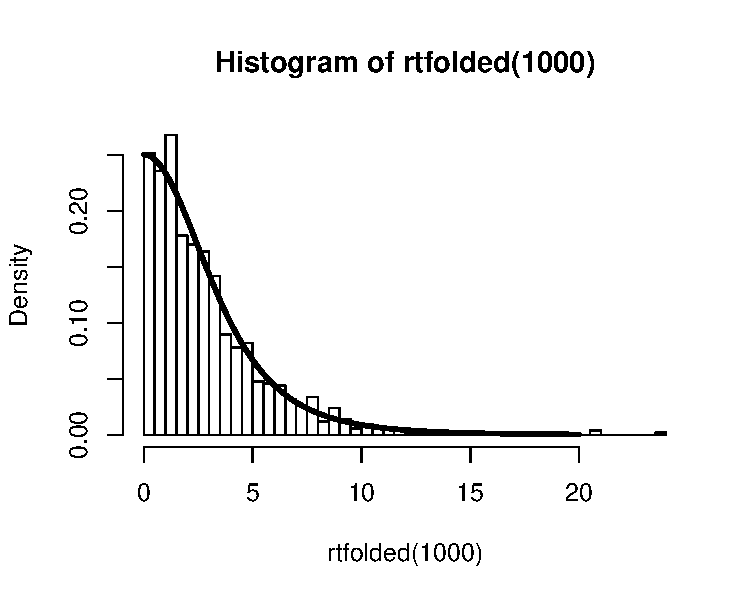
\includegraphics[width=.5\linewidth]{figure/randomdrawsfoldedt} 

\end{knitrout}
\end{center}
\end{singlespace}

\end{enumerate}

\item The basic hierarchical model is:
\begin{align*}
y_{ij} \sim N(\mu+\alpha_j, \sigma^2_y) \\
\alpha_j \sim N(0, \sigma^2_{\alpha})
\end{align*}


\item I used the code below to simulate $y_{ij}$. I first simulated the group effects, and then I simulated individual effects within each group. The code is adapted from your code in \verb+SchoolsFakeData_CompareMethods_F13.R+. The boxplots showing the simulated data are shown below.

\begin{singlespace}
\begin{knitrout}\footnotesize
\definecolor{shadecolor}{rgb}{0.969, 0.969, 0.969}\color{fgcolor}\begin{kframe}
\begin{alltt}
\hlkwd{set.seed}\hlstd{(}\hlnum{10923}\hlstd{)}
 \hlstd{n.j} \hlkwb{<-} \hlkwd{c}\hlstd{(}\hlnum{5}\hlstd{,} \hlnum{10}\hlstd{,} \hlnum{30}\hlstd{,} \hlnum{30}\hlstd{,} \hlnum{20}\hlstd{,} \hlnum{25}\hlstd{,} \hlnum{50}\hlstd{,} \hlnum{10}\hlstd{)}
 \hlstd{n.tot} \hlkwb{<-} \hlkwd{sum}\hlstd{(n.j)}

 \hlstd{J} \hlkwb{<-} \hlnum{8}
 \hlstd{sigma.y} \hlkwb{<-} \hlnum{2}

 \hlstd{mu} \hlkwb{<-} \hlnum{20}
 \hlstd{sigma.alpha} \hlkwb{<-} \hlkwd{sqrt}\hlstd{(}\hlnum{2}\hlstd{)}

\hlstd{alpha} \hlkwb{<-} \hlkwd{numeric}\hlstd{(J)}
\hlkwa{for}\hlstd{(j} \hlkwa{in} \hlnum{1}\hlopt{:}\hlstd{J)\{}
  \hlstd{alpha[j]} \hlkwb{<-} \hlkwd{rnorm}\hlstd{(}\hlnum{1}\hlstd{,} \hlnum{0}\hlstd{,} \hlkwc{sd}\hlstd{=sigma.alpha)}
\hlstd{\}}

 \hlkwd{set.seed}\hlstd{(}\hlnum{2567}\hlstd{)}
 \hlstd{y.ij} \hlkwb{<-} \hlkwd{numeric}\hlstd{(n.tot)}
 \hlstd{school} \hlkwb{<-} \hlkwd{rep}\hlstd{(}\hlnum{NA}\hlstd{,n.tot)}
 \hlstd{n.index} \hlkwb{<-} \hlkwd{c}\hlstd{(}\hlnum{0}\hlstd{,} \hlkwd{cumsum}\hlstd{(n.j))} \hlopt{+}\hlnum{1}
 \hlkwa{for} \hlstd{(j} \hlkwa{in} \hlnum{1}\hlopt{:}\hlstd{J) \{}
   \hlstd{y.ij[n.index[j]}\hlopt{:}\hlstd{(n.index[j}\hlopt{+}\hlnum{1}\hlstd{]}\hlopt{-}\hlnum{1}\hlstd{)]} \hlkwb{<-} \hlkwd{rnorm}\hlstd{(n.j[j],} \hlkwc{mean}\hlstd{=mu}\hlopt{+}\hlstd{alpha[j],} \hlkwc{sd}\hlstd{=sigma.y)}
   \hlstd{school[n.index[j]}\hlopt{:}\hlstd{(n.index[j}\hlopt{+}\hlnum{1}\hlstd{]}\hlopt{-}\hlnum{1}\hlstd{)]} \hlkwb{<-} \hlkwd{rep}\hlstd{(LETTERS[j], n.j[j])}
 \hlstd{\}}
 \hlstd{school} \hlkwb{<-} \hlkwd{factor}\hlstd{(school)}
\end{alltt}
\end{kframe}
\end{knitrout}
\end{singlespace}

\begin{knitrout}\footnotesize
\definecolor{shadecolor}{rgb}{0.969, 0.969, 0.969}\color{fgcolor}
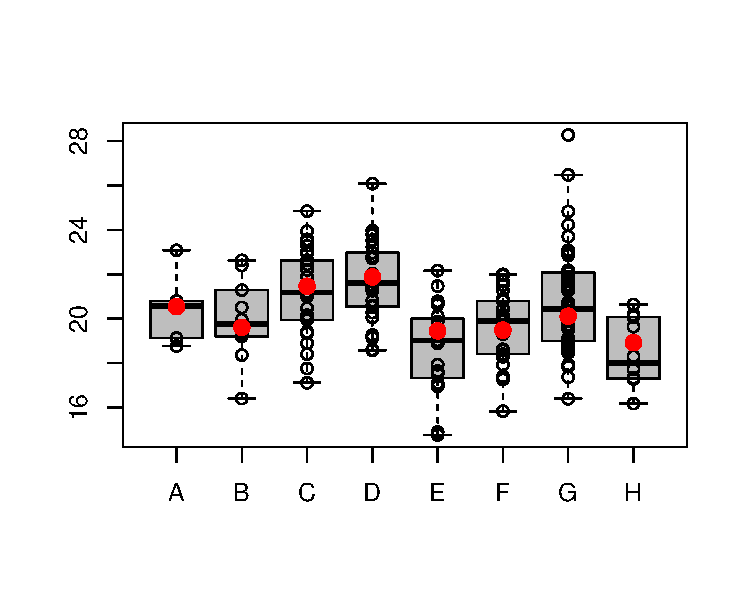
\includegraphics[width=.5\linewidth]{figure/plotsims} 

\end{knitrout}

\item I chose an improper uniform prior for $\mu$, and improper uniform priors for $\sigma_y$ and $\sigma_{\alpha}$ under the constraint that these parameters are larger than $0$.
\begin{align*}
p(\mu) \propto 1 \\
p(\sigma_y) \propto 1 I_{\sigma_y > 0}\\
p(\sigma_{\alpha}) \propto 1 I_{\sigma_{\alpha} > 0}
\end{align*}

\item I chose to use STAN to fit the models. I included model code in the appendix

\begin{enumerate}

\item I chose $\epsilon = 1$ so that an $Inv-Gamma(1, 1)$ prior is used on $\sigma^2_{\alpha}$. Gelman uses this prior in the $2006$ prior, and although it appears to inform the posterior more than the improper uniform prior, it does not influence the posterior nearly as much as the $Gam(0.001, 0.001)$ prior. Additionally, I can't find a symmetric gamma prior that is more diffuse than the $Gam(1,1)$ that does not blow up at $0$. Gelman says he does not recommend using the Inv-Gam($\epsilon$, $\epsilon$) prior when the goal is to inform the posterior as little as  possible.

\begin{center}
\begin{knitrout}\footnotesize
\definecolor{shadecolor}{rgb}{0.969, 0.969, 0.969}\color{fgcolor}
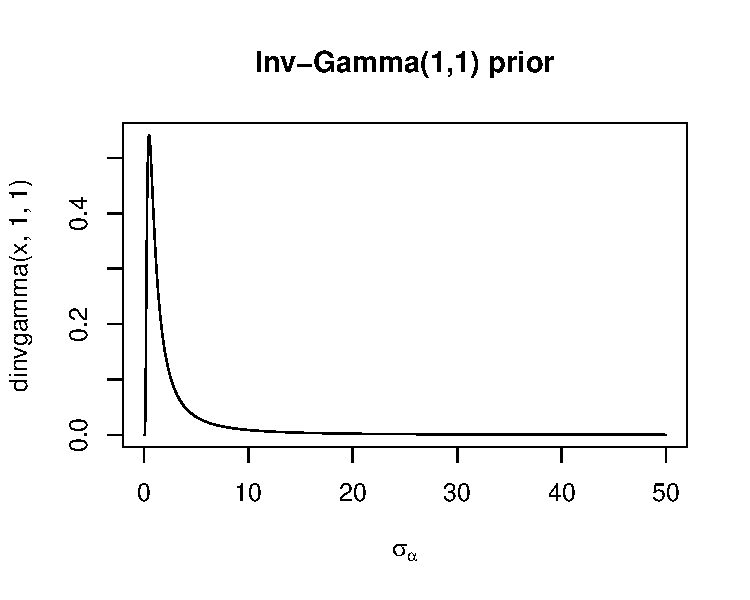
\includegraphics[width=.5\linewidth]{figure/plotdinvgam} 

\end{knitrout}
\end{center}
I just chose a very large number for A, $A=10000$, with the goal of applying a very vague prior on $\sigma^2_{\alpha}$. Normally, I would choose an A that represents a mathematical constraint on the upper bound of $\sigma_{\alpha}$. For example, if I was using the schools example, I would say that a standard deviation of $100$ is a reasonable maximum in the context of SAT scores. But, because I am choosing A for a general hierarchical model with no context, it's hard to choose an upper bound to reflect a natural constraint.









\item Here I compare the posterior distributions of $\sigma_{\alpha}$ obtained from the three priors. The improper uniform prior has the largest range of posterior draws. I would expect this, because it is the most diffuse prior. The $Inv-Gamma(1, 1)$ prior does appear to inform the posterior because the range of posterior draws is the narrowest for this prior. It turns out the $Inv-Gamma(1,1)$ prior is closer to being centered on the true $\sigma_{\alpha}$, $\sqrt{2}$, than any of the other priors. I think this occured by coincidence; the inverse gamma prior happened to put more on values of $\sigma_{\alpha}$ closer to the truth. This was not intentional, however, and I don't think the $Inv-Gam(1,1)$ prior should be thought of as non-informative.

\begin{knitrout}\footnotesize
\definecolor{shadecolor}{rgb}{0.969, 0.969, 0.969}\color{fgcolor}
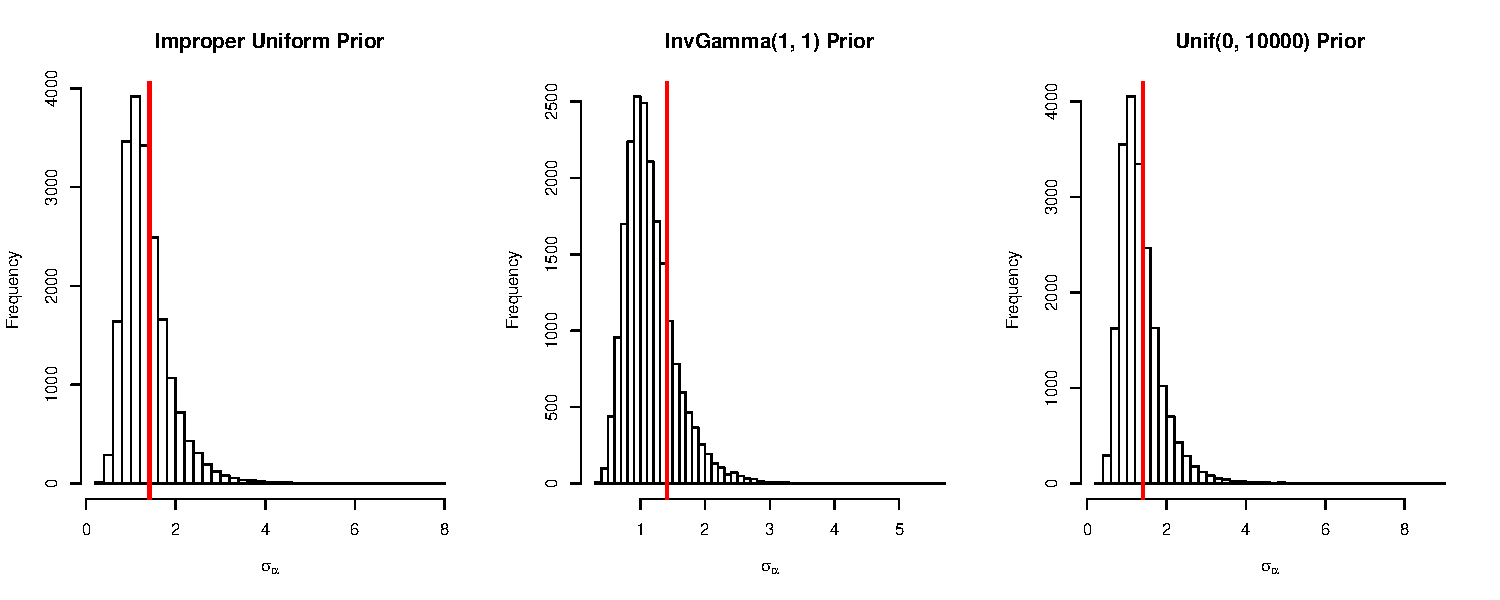
\includegraphics[width=\linewidth]{figure/plotpost} 

\end{knitrout}

\item When looking at the posterior distributions for $\mu$ obtained from the three priors, I noticed they are all centered around $20.5$, just to the right of the true mean of $20$. Results were fairly similar across all three prior distributions, but again we see that the spread of posterior draws for $\mu$ was widest when the uniform priors were used.

\begin{knitrout}\footnotesize
\definecolor{shadecolor}{rgb}{0.969, 0.969, 0.969}\color{fgcolor}
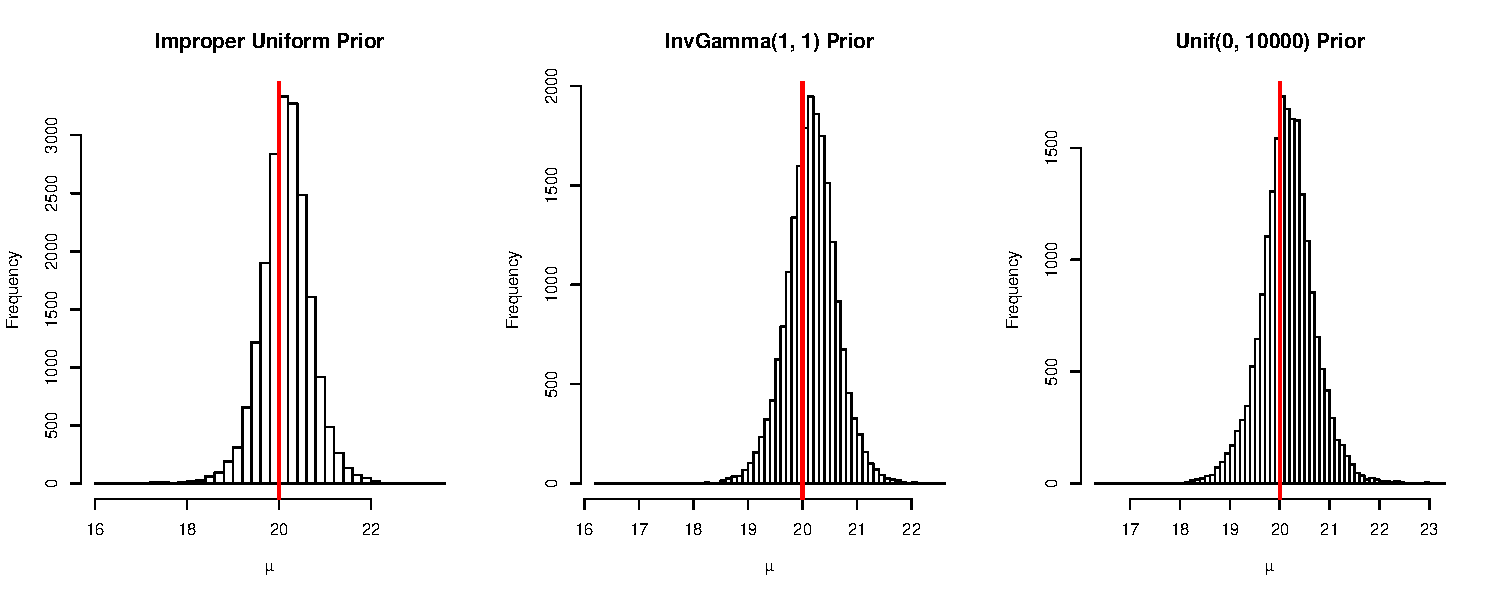
\includegraphics[width=\linewidth]{figure/plotmupost} 

\end{knitrout}

\end{enumerate}

\item The folded $N(0, 100)$ prior has a wider range of posterior draws for $\sigma_{\alpha}$ than the folded Cauchy. The range of posterior $\mu$ values is also slightly larger for the folded $N(0, 100)$. Both posterior distributions for $\mu$ look very similar to the posteriors from all priors in part (e). The posterior for $\sigma_{\alpha}$ from the half Cauchy looks similar to the posterior in part (e) from the inverse Gamma prior. The posterior for $\sigma_{\alpha}$ from the folded normal prior looks similar to the posterior from the uniform priors in (e).


\begin{knitrout}\footnotesize
\definecolor{shadecolor}{rgb}{0.969, 0.969, 0.969}\color{fgcolor}
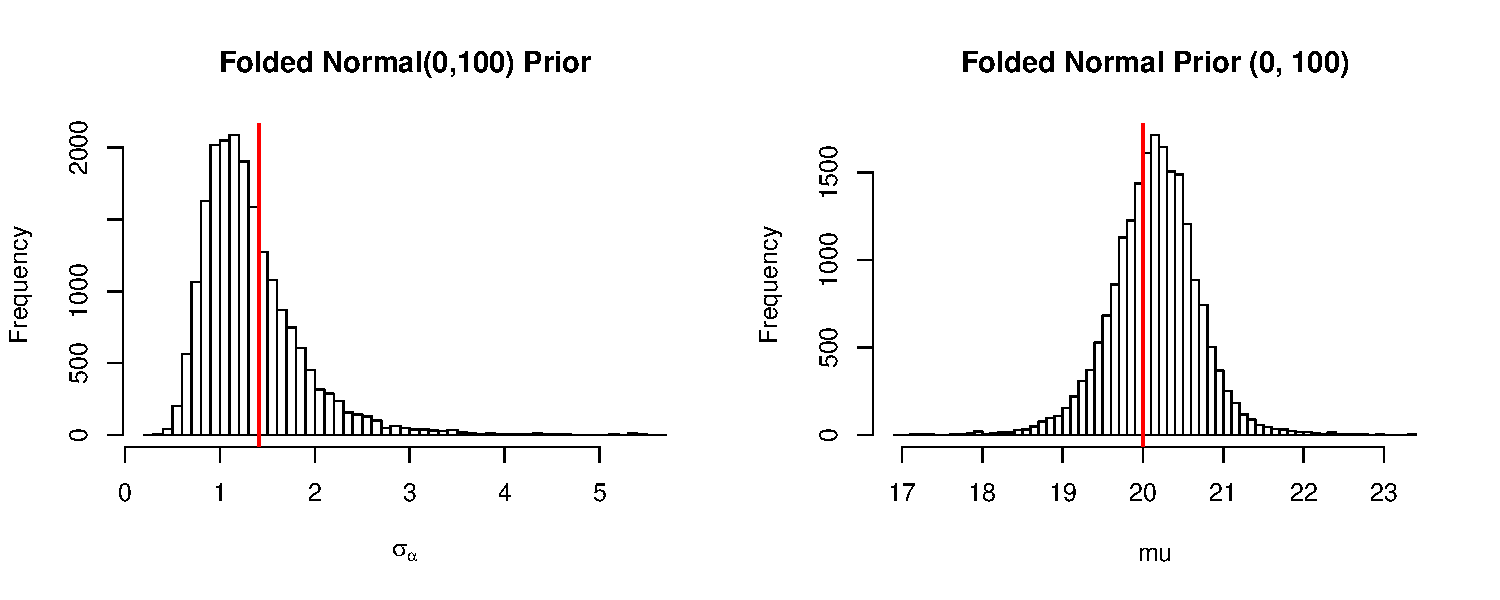
\includegraphics[width=\linewidth]{figure/compare3} 

\end{knitrout}



\begin{knitrout}\footnotesize
\definecolor{shadecolor}{rgb}{0.969, 0.969, 0.969}\color{fgcolor}
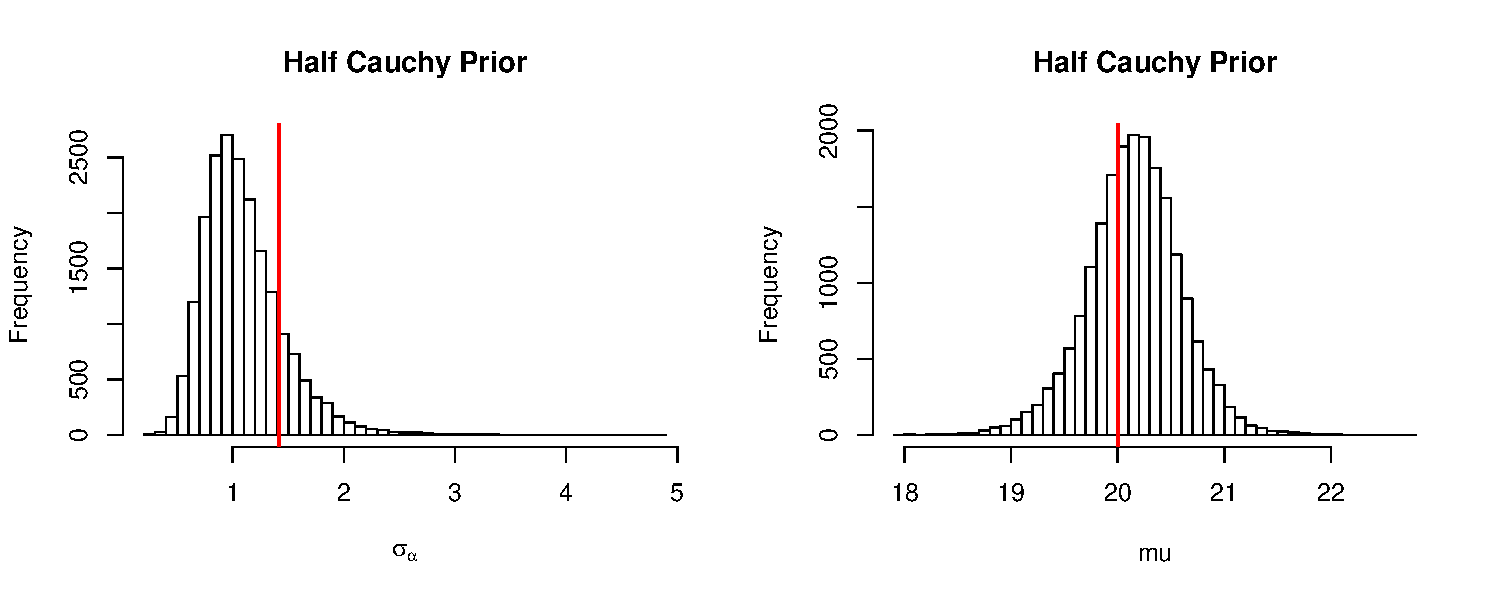
\includegraphics[width=\linewidth]{figure/compare4} 

\end{knitrout}

\end{enumerate}

\item The new simulated data are shown below. I fit the same models as I did in problem $3$ parts (e) and (f).

\begin{singlespace}

\end{singlespace}

\begin{knitrout}\footnotesize
\definecolor{shadecolor}{rgb}{0.969, 0.969, 0.969}\color{fgcolor}
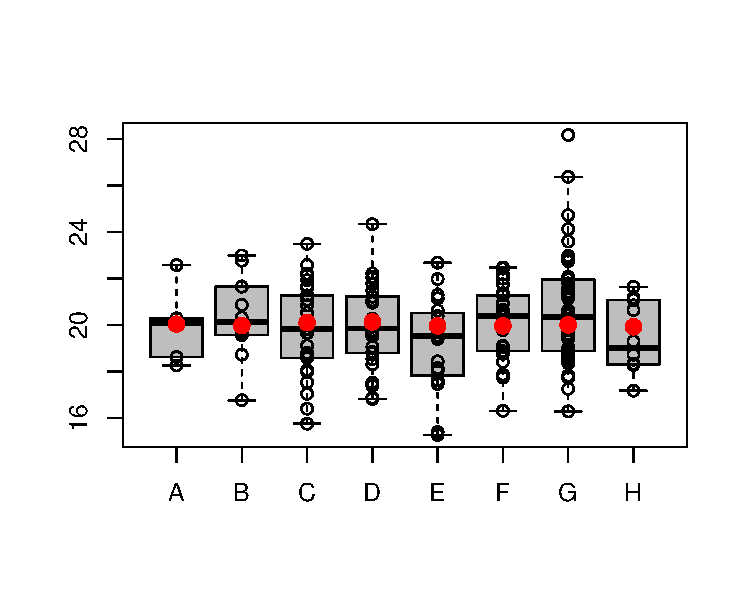
\includegraphics[width=.5\linewidth]{figure/plot4sims} 

\end{knitrout}













Below I plot the posterior distributions for $\mu$ and $\sigma_{\alpha}$ for the different priors. 

\begin{knitrout}\footnotesize
\definecolor{shadecolor}{rgb}{0.969, 0.969, 0.969}\color{fgcolor}
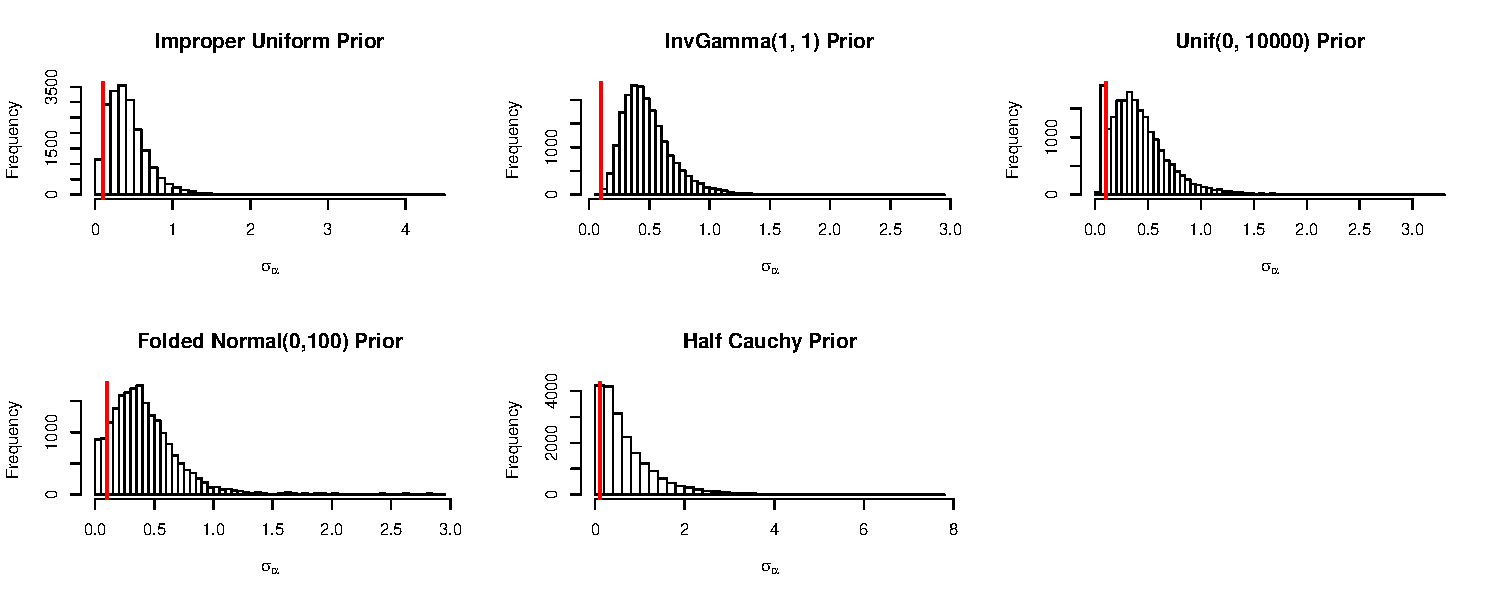
\includegraphics[width=\linewidth]{figure/plotpost4} 

\end{knitrout}


\begin{knitrout}\footnotesize
\definecolor{shadecolor}{rgb}{0.969, 0.969, 0.969}\color{fgcolor}
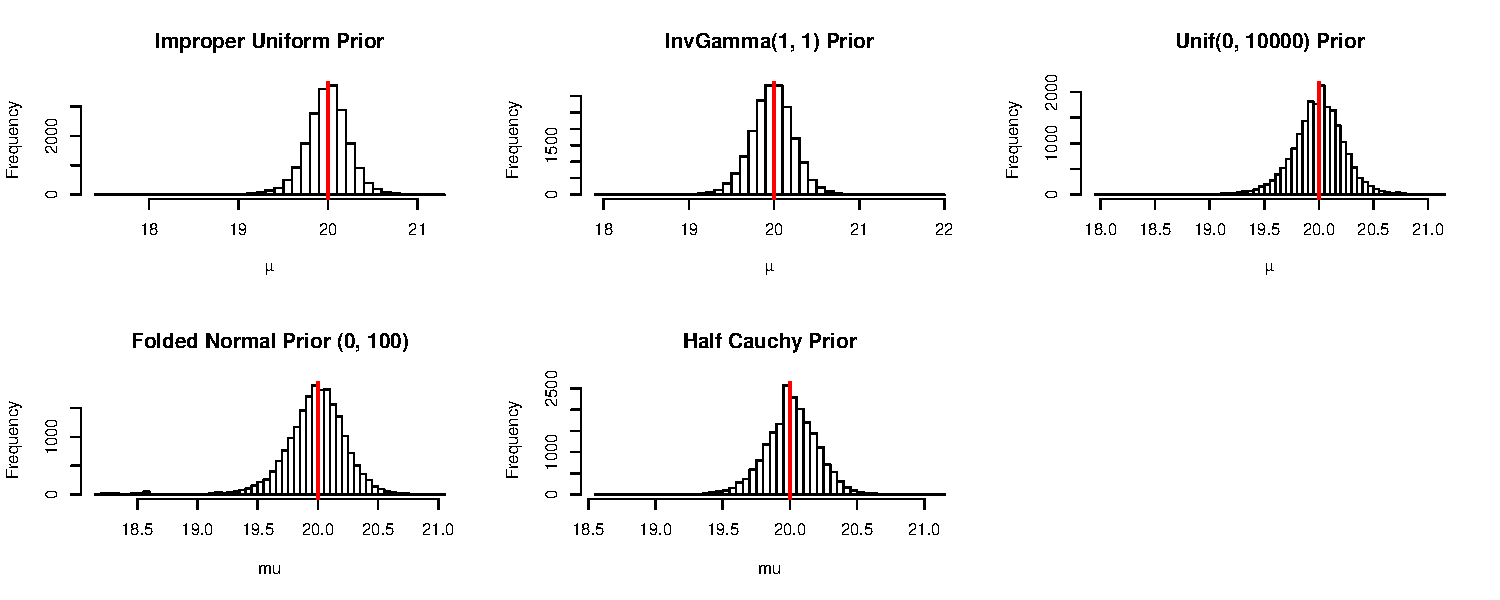
\includegraphics[width=\linewidth]{figure/plotmupost4} 

\end{knitrout}

\begin{enumerate}

\item For all priors, the spreads of the posterior distributions for $\mu$ in problem $4$ are smaller than problem $3$. The posteriors for $\mu$ are still similar across priors, although the folded normal and improper uniform priors still have a wider range of values. \\

The posteriors for $\sigma_{\alpha}$ look very different than they did in problem $3$. Most of them are bumped up against $0$ and centered around $0.5$, quite far from the true value of $0.1$. All of the posteriors have a long right tail, and if the variability were any lower the posterior distributions may turn out to be improper. This is similar to what Gelman points out in section $5$ of his $2006$ paper when the number of groups is small (J=3 rather than J=8), that if the variability among groups is small, or if the number of groups is small, the posterior distributions could turn out to be improper or very sensitive to the prior. In this case, the posteriors for $\sigma_{\alpha}$ end up overestimating the group to group variability because the vague priors used give more density to higher values of $\sigma_{\alpha}$. Gelman says that this is unavoidable due to the asymmetry of the parameter space, but he recommends using the half Cauchy when the variability among groups is low. I do think the results from the half Cauchy look the best, but the posterior draws are still large compared to the true magnitude of $\sigma_{\alpha}$.


%These posterior distributions severely overestimate the variability among the groups, and I'm not sure I'd be comfortable using them for inference.    

\item See caterpillar plots on the next page. In problem $3$, the degree is shrinkage is largest for the inverse gamma prior. I would expect this because the inverse gamma prior puts more density on lower values of $\sigma_{\alpha}$. In the case of problem $4$, however, the degree of shrinkage is largest for the improper uniform prior. I think this occurs because the density of the inverse gamma prior is concentrated above $0.5$. So, in this case, the improper uniform actually has more density on lower values of $\sigma_{\alpha}$ than the inverse gamma prior, resulting in more shrinkage for the improper uniform prior.

The other thing I notice is that there is much more shrinkage overall in the results from problem $4$, but the shrinkage should be more in problem $4$ considering the true standard deviation among groups is only $0.1$. \\

If we were testing for variability among the groups using classical methods, we would find no evidence of variability in problem $4$, but in problem $3$, we would find evidence of variability among the groups. We talked in class about how, with a Bayesian analysis, we don't have to choose between a separate means or a single mean model. But, in problem $4$, the model greatly overestimates the variability among the groups and this seems to be unavoidable. When the variability among groups is small and we know there will be difficulties in estimating the group to group variability, would it be better to use the Bayesian model even though it overestimates variability among groups, or would it be better just to use a single mean model?

\begin{knitrout}\footnotesize
\definecolor{shadecolor}{rgb}{0.969, 0.969, 0.969}\color{fgcolor}
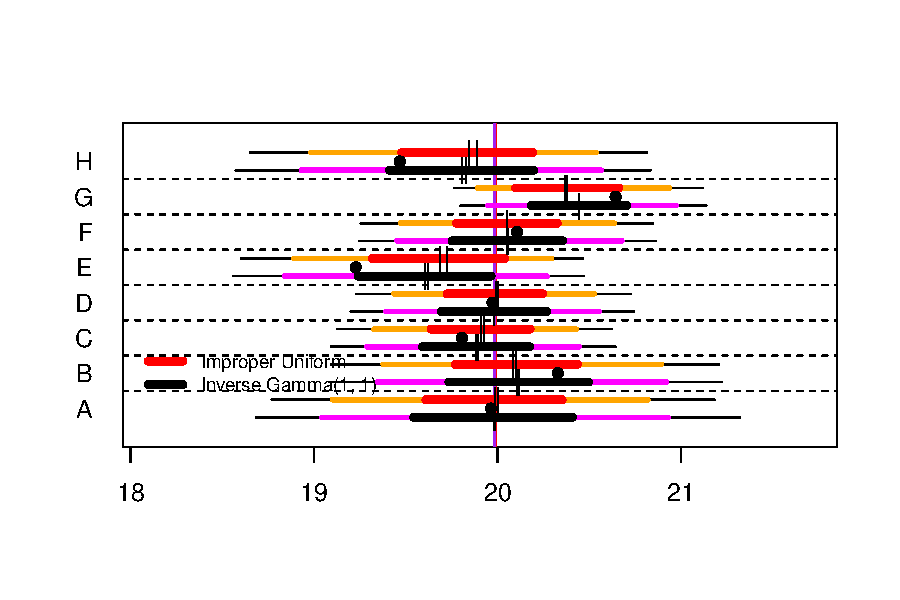
\includegraphics[width=\linewidth]{figure/caterpillarplot4} 

\end{knitrout}

\item Below is the caterpillar plot from problem $3$. See part (b) for my discussion.

\begin{knitrout}\footnotesize
\definecolor{shadecolor}{rgb}{0.969, 0.969, 0.969}\color{fgcolor}
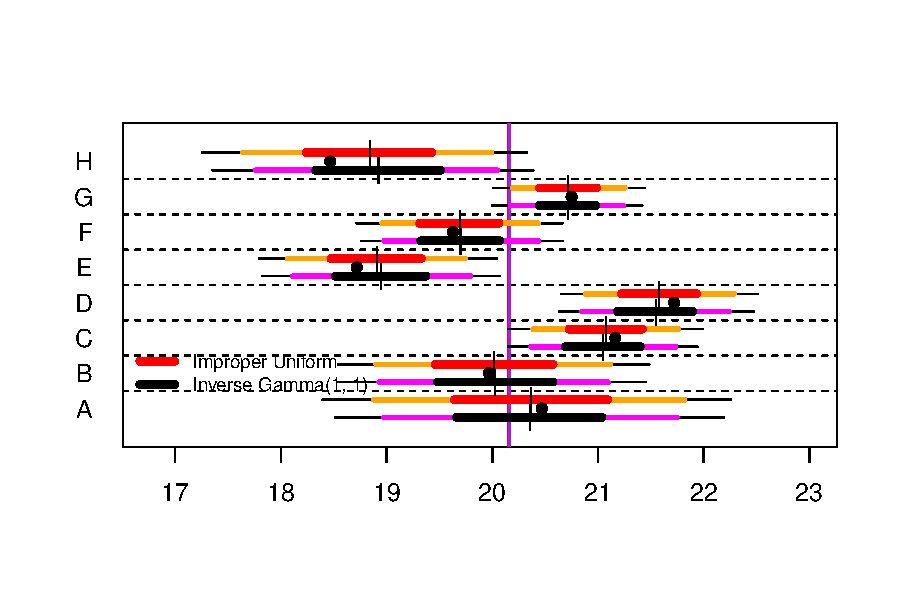
\includegraphics[width=\linewidth]{figure/caterpillarplot3} 

\end{knitrout}

\end{enumerate}

\end{enumerate}

\end{doublespacing}



{\bf \Large R Code Appendix - STAN model code}

\begin{knitrout}\footnotesize
\definecolor{shadecolor}{rgb}{0.969, 0.969, 0.969}\color{fgcolor}\begin{kframe}
\begin{alltt}
\hlcom{###improper uniform prior}
data \{
  int J; 
  real y_1[5]; 
  real y_2[10];
  real y_3[30];
  real y_4[30];
  real y_5[20];
  real y_6[25];
  real y_7[50];
  real y_8[10];
\}

parameters \{
  real mu; 
  real<lower=0> sigma_alpha;
  real<lower=0> sigma_y;
  real alpha[J];
\}

transformed parameters \{
  real theta[J];
  \hlkwd{for} (j in 1:J)
    theta[j] <- mu + alpha[j];
\}

model \{
  alpha ~ \hlkwd{normal}(0, sigma_alpha);
  
  y_1 ~ \hlkwd{normal}(theta[1], sigma_y);
  y_2 ~ \hlkwd{normal}(theta[2], sigma_y);
  y_3 ~ \hlkwd{normal}(theta[3], sigma_y);
  y_4 ~ \hlkwd{normal}(theta[4], sigma_y);
  y_5 ~ \hlkwd{normal}(theta[5], sigma_y);
  y_6 ~ \hlkwd{normal}(theta[6], sigma_y);
  y_7 ~ \hlkwd{normal}(theta[7], sigma_y);
  y_8 ~ \hlkwd{normal}(theta[8], sigma_y); 
\}
\end{alltt}
\end{kframe}
\end{knitrout}

\begin{knitrout}\footnotesize
\definecolor{shadecolor}{rgb}{0.969, 0.969, 0.969}\color{fgcolor}\begin{kframe}
\begin{alltt}
\hlcom{#inverse gamma prior}
data \{
  int J; 
  real y_1[5]; 
  real y_2[10];
  real y_3[30];
  real y_4[30];
  real y_5[20];
  real y_6[25];
  real y_7[50];
  real y_8[10];
\}

parameters \{
  real mu; 
  real<lower=0> sigma_alpha;
  real<lower=0> sigma_y;
  real alpha[J];
\}

transformed parameters \{
  real theta[J];
  \hlkwd{for} (j in 1:J)
    theta[j] <- mu + alpha[j];
\}

model \{
  sigma_alpha ~ \hlkwd{inv_gamma}(1, 1);
  alpha ~ \hlkwd{normal}(0, sigma_alpha);
  
  y_1 ~ \hlkwd{normal}(theta[1], sigma_y);
  y_2 ~ \hlkwd{normal}(theta[2], sigma_y);
  y_3 ~ \hlkwd{normal}(theta[3], sigma_y);
  y_4 ~ \hlkwd{normal}(theta[4], sigma_y);
  y_5 ~ \hlkwd{normal}(theta[5], sigma_y);
  y_6 ~ \hlkwd{normal}(theta[6], sigma_y);
  y_7 ~ \hlkwd{normal}(theta[7], sigma_y);
  y_8 ~ \hlkwd{normal}(theta[8], sigma_y); 
\}
\end{alltt}
\end{kframe}
\end{knitrout}

\begin{knitrout}\footnotesize
\definecolor{shadecolor}{rgb}{0.969, 0.969, 0.969}\color{fgcolor}\begin{kframe}
\begin{alltt}
\hlcom{#proper uniform prior}
data \{
  int J; 
  real y_1[5]; 
  real y_2[10];
  real y_3[30];
  real y_4[30];
  real y_5[20];
  real y_6[25];
  real y_7[50];
  real y_8[10];
\}

parameters \{
  real mu; 
  real<lower=0> sigma_alpha;
  real<lower=0> sigma_y;
  real alpha[J];
\}

transformed parameters \{
  real theta[J];
  \hlkwd{for} (j in 1:J)
    theta[j] <- mu + alpha[j];
\}

model \{
  sigma_alpha ~ \hlkwd{uniform}(0, 10000);
  alpha ~ \hlkwd{normal}(0, sigma_alpha);
  
  y_1 ~ \hlkwd{normal}(theta[1], sigma_y);
  y_2 ~ \hlkwd{normal}(theta[2], sigma_y);
  y_3 ~ \hlkwd{normal}(theta[3], sigma_y);
  y_4 ~ \hlkwd{normal}(theta[4], sigma_y);
  y_5 ~ \hlkwd{normal}(theta[5], sigma_y);
  y_6 ~ \hlkwd{normal}(theta[6], sigma_y);
  y_7 ~ \hlkwd{normal}(theta[7], sigma_y);
  y_8 ~ \hlkwd{normal}(theta[8], sigma_y); 
\}
\end{alltt}
\end{kframe}
\end{knitrout}

\begin{knitrout}\footnotesize
\definecolor{shadecolor}{rgb}{0.969, 0.969, 0.969}\color{fgcolor}\begin{kframe}
\begin{alltt}
\hlcom{#reparameterized with folded normal prior}
data \{
  real sigma_eta;
  int J; 
  real y_1[5]; 
  real y_2[10];
  real y_3[30];
  real y_4[30];
  real y_5[20];
  real y_6[25];
  real y_7[50];
  real y_8[10];
\}

parameters \{
  real mu; 
  real<lower=0> psi;
  real<lower=0> sigma_y;
  real eta[J];
\}

transformed parameters \{
  real theta[J];
  \hlkwd{for} (j in 1:J)
    theta[j] <- mu + psi * eta[j];
\}

model \{
  eta ~ \hlkwd{normal}(0, sigma_eta);
  psi ~ \hlkwd{normal}(0, 100);     
  y_1 ~ \hlkwd{normal}(theta[1], sigma_y);
  y_2 ~ \hlkwd{normal}(theta[2], sigma_y);
  y_3 ~ \hlkwd{normal}(theta[3], sigma_y);
  y_4 ~ \hlkwd{normal}(theta[4], sigma_y);
  y_5 ~ \hlkwd{normal}(theta[5], sigma_y);
  y_6 ~ \hlkwd{normal}(theta[6], sigma_y);
  y_7 ~ \hlkwd{normal}(theta[7], sigma_y);
  y_8 ~ \hlkwd{normal}(theta[8], sigma_y); 
\}
\end{alltt}
\end{kframe}
\end{knitrout}

\begin{knitrout}\footnotesize
\definecolor{shadecolor}{rgb}{0.969, 0.969, 0.969}\color{fgcolor}\begin{kframe}
\begin{alltt}
\hlcom{#reparameterized folded Cauchy}
data \{
  int J; 
  real y_1[5]; 
  real y_2[10];
  real y_3[30];
  real y_4[30];
  real y_5[20];
  real y_6[25];
  real y_7[50];
  real y_8[10];
\}

parameters \{
  real mu; 
  real<lower=0> psi;
  real<lower=0> sigma_y;
  real eta[J];
  real<lower=0> sigma_eta;
\}

transformed parameters \{
  real theta[J];
  \hlkwd{for} (j in 1:J)
    theta[j] <- mu + psi * eta[j];
\}

model \{
  eta ~ \hlkwd{normal}(0, sigma_eta);
  psi ~ \hlkwd{normal}(0, 1);
  sigma_eta ~ \hlkwd{normal}(0, 1);
  y_1 ~ \hlkwd{normal}(theta[1], sigma_y);
  y_2 ~ \hlkwd{normal}(theta[2], sigma_y);
  y_3 ~ \hlkwd{normal}(theta[3], sigma_y);
  y_4 ~ \hlkwd{normal}(theta[4], sigma_y);
  y_5 ~ \hlkwd{normal}(theta[5], sigma_y);
  y_6 ~ \hlkwd{normal}(theta[6], sigma_y);
  y_7 ~ \hlkwd{normal}(theta[7], sigma_y);
  y_8 ~ \hlkwd{normal}(theta[8], sigma_y); 
\}
\end{alltt}
\end{kframe}
\end{knitrout}



\end{document}
